% Created by tikzDevice version 0.12.6 on 2025-02-12 13:11:19
% !TEX encoding = UTF-8 Unicode
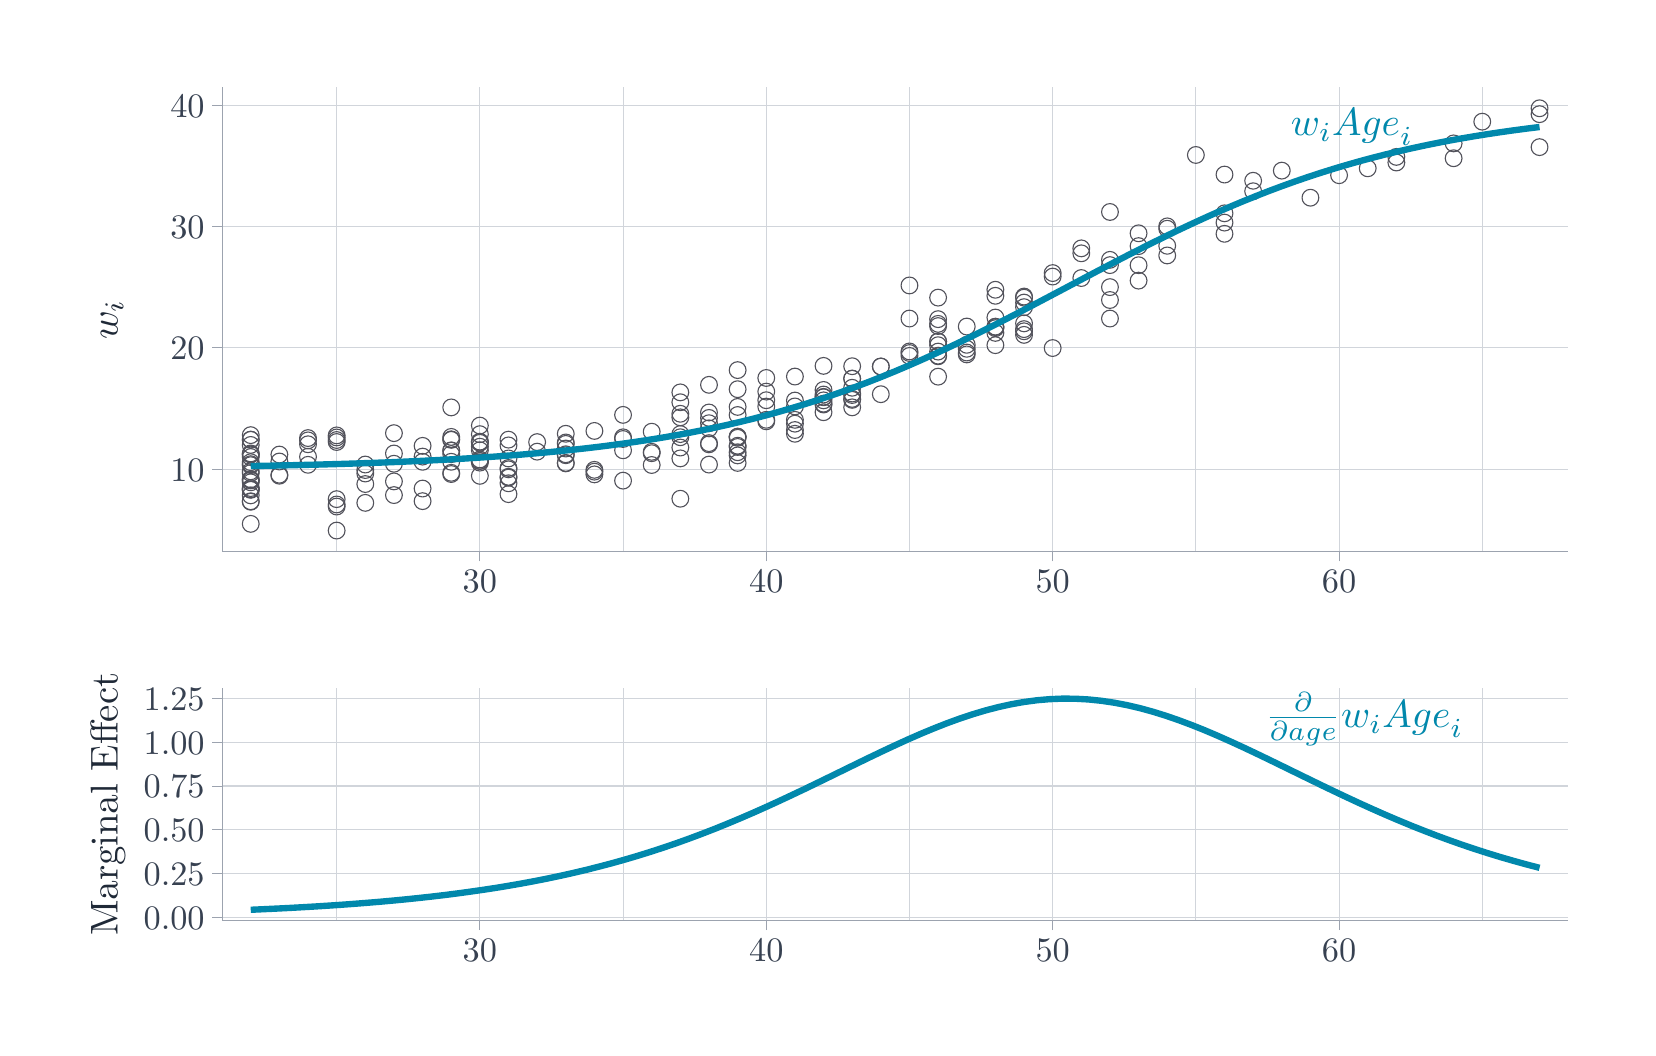
\begin{tikzpicture}[x=1pt,y=1pt]
\definecolor{fillColor}{RGB}{255,255,255}
\path[use as bounding box,fill=fillColor] (0,0) rectangle (578.16,361.35);
\begin{scope}
\path[clip] (  0.00,  0.00) rectangle (578.16,361.35);
\definecolor{drawColor}{RGB}{255,255,255}

\path[draw=drawColor,line width= 0.6pt,line join=round,line cap=round,fill=fillColor] (  0.00, -0.00) rectangle (578.16,361.35);
\end{scope}
\begin{scope}
\path[clip] (  5.50,138.71) rectangle (572.66,355.85);
\definecolor{drawColor}{RGB}{255,255,255}
\definecolor{fillColor}{RGB}{255,255,255}

\path[draw=drawColor,line width= 0.7pt,line join=round,line cap=round,fill=fillColor] (  5.50,138.71) rectangle (572.66,355.85);
\end{scope}
\begin{scope}
\path[clip] (  5.50,  5.50) rectangle (572.66,138.71);
\definecolor{drawColor}{RGB}{255,255,255}
\definecolor{fillColor}{RGB}{255,255,255}

\path[draw=drawColor,line width= 0.7pt,line join=round,line cap=round,fill=fillColor] (  5.50,  5.50) rectangle (572.66,138.71);
\end{scope}
\begin{scope}
\path[clip] ( 70.25,172.00) rectangle (556.66,339.85);
\definecolor{drawColor}{RGB}{255,255,255}
\definecolor{fillColor}{RGB}{255,255,255}

\path[draw=drawColor,line width= 0.7pt,line join=round,line cap=round,fill=fillColor] ( 70.25,172.00) rectangle (556.66,339.85);
\definecolor{drawColor}{RGB}{209,213,219}

\path[draw=drawColor,line width= 0.4pt,line join=round] (111.65,172.00) --
	(111.65,339.85);

\path[draw=drawColor,line width= 0.4pt,line join=round] (215.14,172.00) --
	(215.14,339.85);

\path[draw=drawColor,line width= 0.4pt,line join=round] (318.63,172.00) --
	(318.63,339.85);

\path[draw=drawColor,line width= 0.4pt,line join=round] (422.12,172.00) --
	(422.12,339.85);

\path[draw=drawColor,line width= 0.4pt,line join=round] (525.61,172.00) --
	(525.61,339.85);

\path[draw=drawColor,line width= 0.4pt,line join=round] ( 70.25,201.81) --
	(556.66,201.81);

\path[draw=drawColor,line width= 0.4pt,line join=round] ( 70.25,245.66) --
	(556.66,245.66);

\path[draw=drawColor,line width= 0.4pt,line join=round] ( 70.25,289.51) --
	(556.66,289.51);

\path[draw=drawColor,line width= 0.4pt,line join=round] ( 70.25,333.35) --
	(556.66,333.35);

\path[draw=drawColor,line width= 0.4pt,line join=round] (163.40,172.00) --
	(163.40,339.85);

\path[draw=drawColor,line width= 0.4pt,line join=round] (266.89,172.00) --
	(266.89,339.85);

\path[draw=drawColor,line width= 0.4pt,line join=round] (370.38,172.00) --
	(370.38,339.85);

\path[draw=drawColor,line width= 0.4pt,line join=round] (473.87,172.00) --
	(473.87,339.85);
\definecolor{drawColor}{RGB}{82,82,91}

\path[draw=drawColor,line width= 0.4pt,line join=round,line cap=round] (360.03,252.42) circle (  3.03);

\path[draw=drawColor,line width= 0.4pt,line join=round,line cap=round] (163.40,199.40) circle (  3.03);

\path[draw=drawColor,line width= 0.4pt,line join=round,line cap=round] (194.44,207.20) circle (  3.03);

\path[draw=drawColor,line width= 0.4pt,line join=round,line cap=round] (349.68,246.62) circle (  3.03);

\path[draw=drawColor,line width= 0.4pt,line join=round,line cap=round] (391.08,294.75) circle (  3.03);

\path[draw=drawColor,line width= 0.4pt,line join=round,line cap=round] ( 80.60,203.62) circle (  3.03);

\path[draw=drawColor,line width= 0.4pt,line join=round,line cap=round] ( 80.60,190.04) circle (  3.03);

\path[draw=drawColor,line width= 0.4pt,line join=round,line cap=round] (277.24,219.64) circle (  3.03);

\path[draw=drawColor,line width= 0.4pt,line join=round,line cap=round] (349.68,256.60) circle (  3.03);

\path[draw=drawColor,line width= 0.4pt,line join=round,line cap=round] (370.38,271.41) circle (  3.03);

\path[draw=drawColor,line width= 0.4pt,line join=round,line cap=round] (349.68,252.77) circle (  3.03);

\path[draw=drawColor,line width= 0.4pt,line join=round,line cap=round] (287.58,222.39) circle (  3.03);

\path[draw=drawColor,line width= 0.4pt,line join=round,line cap=round] (256.54,207.93) circle (  3.03);

\path[draw=drawColor,line width= 0.4pt,line join=round,line cap=round] (225.49,207.58) circle (  3.03);

\path[draw=drawColor,line width= 0.4pt,line join=round,line cap=round] (411.77,282.53) circle (  3.03);

\path[draw=drawColor,line width= 0.4pt,line join=round,line cap=round] (194.44,206.85) circle (  3.03);

\path[draw=drawColor,line width= 0.4pt,line join=round,line cap=round] (246.19,218.42) circle (  3.03);

\path[draw=drawColor,line width= 0.4pt,line join=round,line cap=round] (163.40,211.74) circle (  3.03);

\path[draw=drawColor,line width= 0.4pt,line join=round,line cap=round] (246.19,216.55) circle (  3.03);

\path[draw=drawColor,line width= 0.4pt,line join=round,line cap=round] (142.70,194.81) circle (  3.03);

\path[draw=drawColor,line width= 0.4pt,line join=round,line cap=round] (266.89,224.43) circle (  3.03);

\path[draw=drawColor,line width= 0.4pt,line join=round,line cap=round] (328.98,247.94) circle (  3.03);

\path[draw=drawColor,line width= 0.4pt,line join=round,line cap=round] (256.54,213.56) circle (  3.03);

\path[draw=drawColor,line width= 0.4pt,line join=round,line cap=round] (391.08,262.94) circle (  3.03);

\path[draw=drawColor,line width= 0.4pt,line join=round,line cap=round] ( 90.95,207.09) circle (  3.03);

\path[draw=drawColor,line width= 0.4pt,line join=round,line cap=round] (287.58,228.78) circle (  3.03);

\path[draw=drawColor,line width= 0.4pt,line join=round,line cap=round] ( 80.60,206.21) circle (  3.03);

\path[draw=drawColor,line width= 0.4pt,line join=round,line cap=round] (422.12,315.35) circle (  3.03);

\path[draw=drawColor,line width= 0.4pt,line join=round,line cap=round] (308.28,238.91) circle (  3.03);

\path[draw=drawColor,line width= 0.4pt,line join=round,line cap=round] (349.68,264.46) circle (  3.03);

\path[draw=drawColor,line width= 0.4pt,line join=round,line cap=round] (101.30,210.81) circle (  3.03);

\path[draw=drawColor,line width= 0.4pt,line join=round,line cap=round] (349.68,253.32) circle (  3.03);

\path[draw=drawColor,line width= 0.4pt,line join=round,line cap=round] (297.93,229.15) circle (  3.03);

\path[draw=drawColor,line width= 0.4pt,line join=round,line cap=round] (328.98,263.80) circle (  3.03);

\path[draw=drawColor,line width= 0.4pt,line join=round,line cap=round] (132.35,203.77) circle (  3.03);

\path[draw=drawColor,line width= 0.4pt,line join=round,line cap=round] (256.54,210.28) circle (  3.03);

\path[draw=drawColor,line width= 0.4pt,line join=round,line cap=round] (297.93,227.20) circle (  3.03);

\path[draw=drawColor,line width= 0.4pt,line join=round,line cap=round] (391.08,275.55) circle (  3.03);

\path[draw=drawColor,line width= 0.4pt,line join=round,line cap=round] (473.87,308.03) circle (  3.03);

\path[draw=drawColor,line width= 0.4pt,line join=round,line cap=round] (111.65,179.63) circle (  3.03);

\path[draw=drawColor,line width= 0.4pt,line join=round,line cap=round] ( 80.60,200.41) circle (  3.03);

\path[draw=drawColor,line width= 0.4pt,line join=round,line cap=round] (318.63,244.35) circle (  3.03);

\path[draw=drawColor,line width= 0.4pt,line join=round,line cap=round] (235.84,229.56) circle (  3.03);

\path[draw=drawColor,line width= 0.4pt,line join=round,line cap=round] (297.93,226.86) circle (  3.03);

\path[draw=drawColor,line width= 0.4pt,line join=round,line cap=round] (173.74,198.76) circle (  3.03);

\path[draw=drawColor,line width= 0.4pt,line join=round,line cap=round] (235.84,191.13) circle (  3.03);

\path[draw=drawColor,line width= 0.4pt,line join=round,line cap=round] (101.30,206.30) circle (  3.03);

\path[draw=drawColor,line width= 0.4pt,line join=round,line cap=round] (142.70,206.35) circle (  3.03);

\path[draw=drawColor,line width= 0.4pt,line join=round,line cap=round] (380.73,270.88) circle (  3.03);

\path[draw=drawColor,line width= 0.4pt,line join=round,line cap=round] (494.57,314.65) circle (  3.03);

\path[draw=drawColor,line width= 0.4pt,line join=round,line cap=round] (194.44,204.07) circle (  3.03);

\path[draw=drawColor,line width= 0.4pt,line join=round,line cap=round] (515.26,319.53) circle (  3.03);

\path[draw=drawColor,line width= 0.4pt,line join=round,line cap=round] (204.79,200.91) circle (  3.03);

\path[draw=drawColor,line width= 0.4pt,line join=round,line cap=round] (122.00,196.44) circle (  3.03);

\path[draw=drawColor,line width= 0.4pt,line join=round,line cap=round] (297.93,228.61) circle (  3.03);

\path[draw=drawColor,line width= 0.4pt,line join=round,line cap=round] (111.65,212.35) circle (  3.03);

\path[draw=drawColor,line width= 0.4pt,line join=round,line cap=round] (173.74,196.71) circle (  3.03);

\path[draw=drawColor,line width= 0.4pt,line join=round,line cap=round] (173.74,212.48) circle (  3.03);

\path[draw=drawColor,line width= 0.4pt,line join=round,line cap=round] (349.68,251.06) circle (  3.03);

\path[draw=drawColor,line width= 0.4pt,line join=round,line cap=round] (328.98,254.31) circle (  3.03);

\path[draw=drawColor,line width= 0.4pt,line join=round,line cap=round] (339.33,245.31) circle (  3.03);

\path[draw=drawColor,line width= 0.4pt,line join=round,line cap=round] (111.65,190.98) circle (  3.03);

\path[draw=drawColor,line width= 0.4pt,line join=round,line cap=round] (153.05,212.41) circle (  3.03);

\path[draw=drawColor,line width= 0.4pt,line join=round,line cap=round] ( 80.60,190.21) circle (  3.03);

\path[draw=drawColor,line width= 0.4pt,line join=round,line cap=round] (266.89,226.73) circle (  3.03);

\path[draw=drawColor,line width= 0.4pt,line join=round,line cap=round] (277.24,224.48) circle (  3.03);

\path[draw=drawColor,line width= 0.4pt,line join=round,line cap=round] (277.24,235.28) circle (  3.03);

\path[draw=drawColor,line width= 0.4pt,line join=round,line cap=round] (494.57,312.63) circle (  3.03);

\path[draw=drawColor,line width= 0.4pt,line join=round,line cap=round] (266.89,229.84) circle (  3.03);

\path[draw=drawColor,line width= 0.4pt,line join=round,line cap=round] (111.65,214.02) circle (  3.03);

\path[draw=drawColor,line width= 0.4pt,line join=round,line cap=round] (546.31,330.09) circle (  3.03);

\path[draw=drawColor,line width= 0.4pt,line join=round,line cap=round] (235.84,214.49) circle (  3.03);

\path[draw=drawColor,line width= 0.4pt,line join=round,line cap=round] (132.35,214.83) circle (  3.03);

\path[draw=drawColor,line width= 0.4pt,line join=round,line cap=round] (287.58,239.14) circle (  3.03);

\path[draw=drawColor,line width= 0.4pt,line join=round,line cap=round] (153.05,208.49) circle (  3.03);

\path[draw=drawColor,line width= 0.4pt,line join=round,line cap=round] (246.19,222.29) circle (  3.03);

\path[draw=drawColor,line width= 0.4pt,line join=round,line cap=round] ( 80.60,204.34) circle (  3.03);

\path[draw=drawColor,line width= 0.4pt,line join=round,line cap=round] ( 80.60,197.06) circle (  3.03);

\path[draw=drawColor,line width= 0.4pt,line join=round,line cap=round] (360.03,263.78) circle (  3.03);

\path[draw=drawColor,line width= 0.4pt,line join=round,line cap=round] (546.31,318.18) circle (  3.03);

\path[draw=drawColor,line width= 0.4pt,line join=round,line cap=round] (204.79,199.93) circle (  3.03);

\path[draw=drawColor,line width= 0.4pt,line join=round,line cap=round] ( 80.60,197.76) circle (  3.03);

\path[draw=drawColor,line width= 0.4pt,line join=round,line cap=round] (204.79,201.57) circle (  3.03);

\path[draw=drawColor,line width= 0.4pt,line join=round,line cap=round] (215.14,208.63) circle (  3.03);

\path[draw=drawColor,line width= 0.4pt,line join=round,line cap=round] (349.68,266.64) circle (  3.03);

\path[draw=drawColor,line width= 0.4pt,line join=round,line cap=round] (401.42,275.51) circle (  3.03);

\path[draw=drawColor,line width= 0.4pt,line join=round,line cap=round] (328.98,253.52) circle (  3.03);

\path[draw=drawColor,line width= 0.4pt,line join=round,line cap=round] ( 80.60,212.43) circle (  3.03);

\path[draw=drawColor,line width= 0.4pt,line join=round,line cap=round] (173.74,199.06) circle (  3.03);

\path[draw=drawColor,line width= 0.4pt,line join=round,line cap=round] (215.14,221.43) circle (  3.03);

\path[draw=drawColor,line width= 0.4pt,line join=round,line cap=round] (339.33,253.35) circle (  3.03);

\path[draw=drawColor,line width= 0.4pt,line join=round,line cap=round] (132.35,197.39) circle (  3.03);

\path[draw=drawColor,line width= 0.4pt,line join=round,line cap=round] (142.70,190.26) circle (  3.03);

\path[draw=drawColor,line width= 0.4pt,line join=round,line cap=round] (256.54,213.52) circle (  3.03);

\path[draw=drawColor,line width= 0.4pt,line join=round,line cap=round] (204.79,215.63) circle (  3.03);

\path[draw=drawColor,line width= 0.4pt,line join=round,line cap=round] (277.24,214.60) circle (  3.03);

\path[draw=drawColor,line width= 0.4pt,line join=round,line cap=round] (173.74,201.75) circle (  3.03);

\path[draw=drawColor,line width= 0.4pt,line join=round,line cap=round] (432.47,294.26) circle (  3.03);

\path[draw=drawColor,line width= 0.4pt,line join=round,line cap=round] (287.58,225.18) circle (  3.03);

\path[draw=drawColor,line width= 0.4pt,line join=round,line cap=round] (101.30,203.39) circle (  3.03);

\path[draw=drawColor,line width= 0.4pt,line join=round,line cap=round] (411.77,289.55) circle (  3.03);

\path[draw=drawColor,line width= 0.4pt,line join=round,line cap=round] (235.84,220.54) circle (  3.03);

\path[draw=drawColor,line width= 0.4pt,line join=round,line cap=round] (101.30,213.05) circle (  3.03);

\path[draw=drawColor,line width= 0.4pt,line join=round,line cap=round] ( 90.95,204.58) circle (  3.03);

\path[draw=drawColor,line width= 0.4pt,line join=round,line cap=round] (401.42,282.42) circle (  3.03);

\path[draw=drawColor,line width= 0.4pt,line join=round,line cap=round] (163.40,211.34) circle (  3.03);

\path[draw=drawColor,line width= 0.4pt,line join=round,line cap=round] (360.03,254.50) circle (  3.03);

\path[draw=drawColor,line width= 0.4pt,line join=round,line cap=round] (297.93,231.23) circle (  3.03);

\path[draw=drawColor,line width= 0.4pt,line join=round,line cap=round] (266.89,219.65) circle (  3.03);

\path[draw=drawColor,line width= 0.4pt,line join=round,line cap=round] (453.17,309.69) circle (  3.03);

\path[draw=drawColor,line width= 0.4pt,line join=round,line cap=round] (380.73,279.81) circle (  3.03);

\path[draw=drawColor,line width= 0.4pt,line join=round,line cap=round] ( 80.60,207.50) circle (  3.03);

\path[draw=drawColor,line width= 0.4pt,line join=round,line cap=round] (256.54,221.38) circle (  3.03);

\path[draw=drawColor,line width= 0.4pt,line join=round,line cap=round] ( 80.60,194.99) circle (  3.03);

\path[draw=drawColor,line width= 0.4pt,line join=round,line cap=round] (328.98,256.02) circle (  3.03);

\path[draw=drawColor,line width= 0.4pt,line join=round,line cap=round] (256.54,206.79) circle (  3.03);

\path[draw=drawColor,line width= 0.4pt,line join=round,line cap=round] (122.00,200.25) circle (  3.03);

\path[draw=drawColor,line width= 0.4pt,line join=round,line cap=round] (163.40,205.31) circle (  3.03);

\path[draw=drawColor,line width= 0.4pt,line join=round,line cap=round] (391.08,277.45) circle (  3.03);

\path[draw=drawColor,line width= 0.4pt,line join=round,line cap=round] ( 90.95,199.81) circle (  3.03);

\path[draw=drawColor,line width= 0.4pt,line join=round,line cap=round] (297.93,234.50) circle (  3.03);

\path[draw=drawColor,line width= 0.4pt,line join=round,line cap=round] (339.33,243.28) circle (  3.03);

\path[draw=drawColor,line width= 0.4pt,line join=round,line cap=round] (380.73,281.60) circle (  3.03);

\path[draw=drawColor,line width= 0.4pt,line join=round,line cap=round] (235.84,225.99) circle (  3.03);

\path[draw=drawColor,line width= 0.4pt,line join=round,line cap=round] (215.14,212.72) circle (  3.03);

\path[draw=drawColor,line width= 0.4pt,line join=round,line cap=round] (266.89,234.77) circle (  3.03);

\path[draw=drawColor,line width= 0.4pt,line join=round,line cap=round] (153.05,224.13) circle (  3.03);

\path[draw=drawColor,line width= 0.4pt,line join=round,line cap=round] (391.08,267.60) circle (  3.03);

\path[draw=drawColor,line width= 0.4pt,line join=round,line cap=round] (442.82,306.03) circle (  3.03);

\path[draw=drawColor,line width= 0.4pt,line join=round,line cap=round] (463.52,299.90) circle (  3.03);

\path[draw=drawColor,line width= 0.4pt,line join=round,line cap=round] (111.65,213.27) circle (  3.03);

\path[draw=drawColor,line width= 0.4pt,line join=round,line cap=round] (370.38,272.67) circle (  3.03);

\path[draw=drawColor,line width= 0.4pt,line join=round,line cap=round] (328.98,246.61) circle (  3.03);

\path[draw=drawColor,line width= 0.4pt,line join=round,line cap=round] (349.68,253.15) circle (  3.03);

\path[draw=drawColor,line width= 0.4pt,line join=round,line cap=round] ( 80.60,182.05) circle (  3.03);

\path[draw=drawColor,line width= 0.4pt,line join=round,line cap=round] ( 80.60,194.36) circle (  3.03);

\path[draw=drawColor,line width= 0.4pt,line join=round,line cap=round] (266.89,219.10) circle (  3.03);

\path[draw=drawColor,line width= 0.4pt,line join=round,line cap=round] (308.28,238.89) circle (  3.03);

\path[draw=drawColor,line width= 0.4pt,line join=round,line cap=round] (411.77,288.70) circle (  3.03);

\path[draw=drawColor,line width= 0.4pt,line join=round,line cap=round] (297.93,234.55) circle (  3.03);

\path[draw=drawColor,line width= 0.4pt,line join=round,line cap=round] (287.58,227.94) circle (  3.03);

\path[draw=drawColor,line width= 0.4pt,line join=round,line cap=round] (163.40,214.46) circle (  3.03);

\path[draw=drawColor,line width= 0.4pt,line join=round,line cap=round] (246.19,211.22) circle (  3.03);

\path[draw=drawColor,line width= 0.4pt,line join=round,line cap=round] (111.65,189.05) circle (  3.03);

\path[draw=drawColor,line width= 0.4pt,line join=round,line cap=round] (360.03,251.64) circle (  3.03);

\path[draw=drawColor,line width= 0.4pt,line join=round,line cap=round] (484.22,310.53) circle (  3.03);

\path[draw=drawColor,line width= 0.4pt,line join=round,line cap=round] (256.54,230.71) circle (  3.03);

\path[draw=drawColor,line width= 0.4pt,line join=round,line cap=round] (153.05,204.48) circle (  3.03);

\path[draw=drawColor,line width= 0.4pt,line join=round,line cap=round] (287.58,226.68) circle (  3.03);

\path[draw=drawColor,line width= 0.4pt,line join=round,line cap=round] ( 80.60,212.49) circle (  3.03);

\path[draw=drawColor,line width= 0.4pt,line join=round,line cap=round] (318.63,268.20) circle (  3.03);

\path[draw=drawColor,line width= 0.4pt,line join=round,line cap=round] (297.93,239.01) circle (  3.03);

\path[draw=drawColor,line width= 0.4pt,line join=round,line cap=round] (339.33,246.75) circle (  3.03);

\path[draw=drawColor,line width= 0.4pt,line join=round,line cap=round] (370.38,245.58) circle (  3.03);

\path[draw=drawColor,line width= 0.4pt,line join=round,line cap=round] (277.24,215.96) circle (  3.03);

\path[draw=drawColor,line width= 0.4pt,line join=round,line cap=round] (256.54,237.61) circle (  3.03);

\path[draw=drawColor,line width= 0.4pt,line join=round,line cap=round] (215.14,197.67) circle (  3.03);

\path[draw=drawColor,line width= 0.4pt,line join=round,line cap=round] (111.65,188.31) circle (  3.03);

\path[draw=drawColor,line width= 0.4pt,line join=round,line cap=round] (153.05,207.25) circle (  3.03);

\path[draw=drawColor,line width= 0.4pt,line join=round,line cap=round] (184.09,211.59) circle (  3.03);

\path[draw=drawColor,line width= 0.4pt,line join=round,line cap=round] (328.98,235.24) circle (  3.03);

\path[draw=drawColor,line width= 0.4pt,line join=round,line cap=round] (360.03,250.34) circle (  3.03);

\path[draw=drawColor,line width= 0.4pt,line join=round,line cap=round] ( 80.60,203.25) circle (  3.03);

\path[draw=drawColor,line width= 0.4pt,line join=round,line cap=round] ( 80.60,194.45) circle (  3.03);

\path[draw=drawColor,line width= 0.4pt,line join=round,line cap=round] (297.93,224.15) circle (  3.03);

\path[draw=drawColor,line width= 0.4pt,line join=round,line cap=round] (432.47,286.86) circle (  3.03);

\path[draw=drawColor,line width= 0.4pt,line join=round,line cap=round] (277.24,218.25) circle (  3.03);

\path[draw=drawColor,line width= 0.4pt,line join=round,line cap=round] (122.00,203.49) circle (  3.03);

\path[draw=drawColor,line width= 0.4pt,line join=round,line cap=round] (163.40,204.81) circle (  3.03);

\path[draw=drawColor,line width= 0.4pt,line join=round,line cap=round] (525.61,327.38) circle (  3.03);

\path[draw=drawColor,line width= 0.4pt,line join=round,line cap=round] (142.70,204.47) circle (  3.03);

\path[draw=drawColor,line width= 0.4pt,line join=round,line cap=round] (401.42,269.94) circle (  3.03);

\path[draw=drawColor,line width= 0.4pt,line join=round,line cap=round] ( 80.60,207.13) circle (  3.03);

\path[draw=drawColor,line width= 0.4pt,line join=round,line cap=round] (132.35,207.48) circle (  3.03);

\path[draw=drawColor,line width= 0.4pt,line join=round,line cap=round] (287.58,227.79) circle (  3.03);

\path[draw=drawColor,line width= 0.4pt,line join=round,line cap=round] (235.84,209.63) circle (  3.03);

\path[draw=drawColor,line width= 0.4pt,line join=round,line cap=round] (173.74,202.24) circle (  3.03);

\path[draw=drawColor,line width= 0.4pt,line join=round,line cap=round] (401.42,287.04) circle (  3.03);

\path[draw=drawColor,line width= 0.4pt,line join=round,line cap=round] (287.58,230.44) circle (  3.03);

\path[draw=drawColor,line width= 0.4pt,line join=round,line cap=round] (163.40,211.68) circle (  3.03);

\path[draw=drawColor,line width= 0.4pt,line join=round,line cap=round] (153.05,213.47) circle (  3.03);

\path[draw=drawColor,line width= 0.4pt,line join=round,line cap=round] (360.03,264.19) circle (  3.03);

\path[draw=drawColor,line width= 0.4pt,line join=round,line cap=round] (111.65,211.63) circle (  3.03);

\path[draw=drawColor,line width= 0.4pt,line join=round,line cap=round] (184.09,208.14) circle (  3.03);

\path[draw=drawColor,line width= 0.4pt,line join=round,line cap=round] (339.33,243.96) circle (  3.03);

\path[draw=drawColor,line width= 0.4pt,line join=round,line cap=round] (442.82,302.24) circle (  3.03);

\path[draw=drawColor,line width= 0.4pt,line join=round,line cap=round] (194.44,203.91) circle (  3.03);

\path[draw=drawColor,line width= 0.4pt,line join=round,line cap=round] (153.05,200.50) circle (  3.03);

\path[draw=drawColor,line width= 0.4pt,line join=round,line cap=round] (225.49,215.35) circle (  3.03);

\path[draw=drawColor,line width= 0.4pt,line join=round,line cap=round] (256.54,209.85) circle (  3.03);

\path[draw=drawColor,line width= 0.4pt,line join=round,line cap=round] (246.19,210.78) circle (  3.03);

\path[draw=drawColor,line width= 0.4pt,line join=round,line cap=round] (256.54,224.31) circle (  3.03);

\path[draw=drawColor,line width= 0.4pt,line join=round,line cap=round] (101.30,212.22) circle (  3.03);

\path[draw=drawColor,line width= 0.4pt,line join=round,line cap=round] ( 90.95,199.45) circle (  3.03);

\path[draw=drawColor,line width= 0.4pt,line join=round,line cap=round] (256.54,204.07) circle (  3.03);

\path[draw=drawColor,line width= 0.4pt,line join=round,line cap=round] (328.98,247.95) circle (  3.03);

\path[draw=drawColor,line width= 0.4pt,line join=round,line cap=round] (163.40,209.94) circle (  3.03);

\path[draw=drawColor,line width= 0.4pt,line join=round,line cap=round] (173.74,210.40) circle (  3.03);

\path[draw=drawColor,line width= 0.4pt,line join=round,line cap=round] (277.24,226.61) circle (  3.03);

\path[draw=drawColor,line width= 0.4pt,line join=round,line cap=round] (318.63,256.24) circle (  3.03);

\path[draw=drawColor,line width= 0.4pt,line join=round,line cap=round] (132.35,192.45) circle (  3.03);

\path[draw=drawColor,line width= 0.4pt,line join=round,line cap=round] (225.49,208.08) circle (  3.03);

\path[draw=drawColor,line width= 0.4pt,line join=round,line cap=round] (318.63,243.78) circle (  3.03);

\path[draw=drawColor,line width= 0.4pt,line join=round,line cap=round] (256.54,213.15) circle (  3.03);

\path[draw=drawColor,line width= 0.4pt,line join=round,line cap=round] (360.03,260.35) circle (  3.03);

\path[draw=drawColor,line width= 0.4pt,line join=round,line cap=round] (163.40,217.56) circle (  3.03);

\path[draw=drawColor,line width= 0.4pt,line join=round,line cap=round] (153.05,200.06) circle (  3.03);

\path[draw=drawColor,line width= 0.4pt,line join=round,line cap=round] (142.70,210.24) circle (  3.03);

\path[draw=drawColor,line width= 0.4pt,line join=round,line cap=round] (153.05,208.61) circle (  3.03);

\path[draw=drawColor,line width= 0.4pt,line join=round,line cap=round] (225.49,203.32) circle (  3.03);

\path[draw=drawColor,line width= 0.4pt,line join=round,line cap=round] (411.77,279.04) circle (  3.03);

\path[draw=drawColor,line width= 0.4pt,line join=round,line cap=round] ( 80.60,198.16) circle (  3.03);

\path[draw=drawColor,line width= 0.4pt,line join=round,line cap=round] ( 80.60,214.11) circle (  3.03);

\path[draw=drawColor,line width= 0.4pt,line join=round,line cap=round] (122.00,189.64) circle (  3.03);

\path[draw=drawColor,line width= 0.4pt,line join=round,line cap=round] (360.03,262.01) circle (  3.03);

\path[draw=drawColor,line width= 0.4pt,line join=round,line cap=round] (246.19,203.47) circle (  3.03);

\path[draw=drawColor,line width= 0.4pt,line join=round,line cap=round] (328.98,244.30) circle (  3.03);

\path[draw=drawColor,line width= 0.4pt,line join=round,line cap=round] (546.31,332.22) circle (  3.03);

\path[draw=drawColor,line width= 0.4pt,line join=round,line cap=round] (194.44,211.46) circle (  3.03);

\path[draw=drawColor,line width= 0.4pt,line join=round,line cap=round] (173.74,205.68) circle (  3.03);

\path[draw=drawColor,line width= 0.4pt,line join=round,line cap=round] (246.19,220.33) circle (  3.03);

\path[draw=drawColor,line width= 0.4pt,line join=round,line cap=round] (235.84,221.83) circle (  3.03);

\path[draw=drawColor,line width= 0.4pt,line join=round,line cap=round] (194.44,214.60) circle (  3.03);

\path[draw=drawColor,line width= 0.4pt,line join=round,line cap=round] (308.28,228.90) circle (  3.03);

\path[draw=drawColor,line width= 0.4pt,line join=round,line cap=round] ( 80.60,201.04) circle (  3.03);

\path[draw=drawColor,line width= 0.4pt,line join=round,line cap=round] (318.63,242.74) circle (  3.03);

\path[draw=drawColor,line width= 0.4pt,line join=round,line cap=round] (163.40,208.65) circle (  3.03);

\path[draw=drawColor,line width= 0.4pt,line join=round,line cap=round] ( 80.60,197.87) circle (  3.03);

\path[draw=drawColor,line width= 0.4pt,line join=round,line cap=round] (122.00,201.50) circle (  3.03);

\path[draw=drawColor,line width= 0.4pt,line join=round,line cap=round] ( 80.60,207.15) circle (  3.03);

\path[draw=drawColor,line width= 0.4pt,line join=round,line cap=round] (246.19,232.29) circle (  3.03);

\path[draw=drawColor,line width= 0.4pt,line join=round,line cap=round] (235.84,213.35) circle (  3.03);

\path[draw=drawColor,line width= 0.4pt,line join=round,line cap=round] ( 80.60,194.57) circle (  3.03);

\path[draw=drawColor,line width= 0.4pt,line join=round,line cap=round] (328.98,242.60) circle (  3.03);

\path[draw=drawColor,line width= 0.4pt,line join=round,line cap=round] (432.47,290.91) circle (  3.03);

\path[draw=drawColor,line width= 0.4pt,line join=round,line cap=round] (515.26,314.16) circle (  3.03);

\path[draw=drawColor,line width= 0.4pt,line join=round,line cap=round] (391.08,256.24) circle (  3.03);

\path[draw=drawColor,line width= 0.4pt,line join=round,line cap=round] (432.47,308.27) circle (  3.03);

\path[draw=drawColor,line width= 0.4pt,line join=round,line cap=round] (194.44,210.95) circle (  3.03);

\path[draw=drawColor,line width= 0.4pt,line join=round,line cap=round] (163.40,204.18) circle (  3.03);

\path[draw=drawColor,line width= 0.4pt,line join=round,line cap=round] ( 80.60,210.57) circle (  3.03);

\path[draw=drawColor,line width= 0.4pt,line join=round,line cap=round] (287.58,225.49) circle (  3.03);

\path[draw=drawColor,line width= 0.4pt,line join=round,line cap=round] (235.84,205.71) circle (  3.03);

\path[draw=drawColor,line width= 0.4pt,line join=round,line cap=round] (163.40,204.76) circle (  3.03);

\path[draw=drawColor,line width= 0.4pt,line join=round,line cap=round] (215.14,213.32) circle (  3.03);

\path[draw=drawColor,line width= 0.4pt,line join=round,line cap=round] (173.74,192.79) circle (  3.03);

\path[draw=drawColor,line width= 0.4pt,line join=round,line cap=round] (328.98,242.83) circle (  3.03);

\path[draw=drawColor,line width= 0.4pt,line join=round,line cap=round] (153.05,212.59) circle (  3.03);

\path[draw=drawColor,line width= 0.4pt,line join=round,line cap=round] (194.44,209.27) circle (  3.03);

\path[draw=drawColor,line width= 0.4pt,line join=round,line cap=round] ( 80.60,192.35) circle (  3.03);
\definecolor{drawColor}{RGB}{1,136,172}

\path[draw=drawColor,line width= 2.3pt,line join=round] ( 80.60,202.94) --
	( 85.26,203.02) --
	( 89.92,203.12) --
	( 94.57,203.22) --
	( 99.23,203.33) --
	(103.89,203.44) --
	(108.55,203.57) --
	(113.20,203.70) --
	(117.86,203.85) --
	(122.52,204.01) --
	(127.17,204.17) --
	(131.83,204.35) --
	(136.49,204.55) --
	(141.15,204.76) --
	(145.80,204.98) --
	(150.46,205.22) --
	(155.12,205.48) --
	(159.77,205.76) --
	(164.43,206.06) --
	(169.09,206.38) --
	(173.74,206.72) --
	(178.40,207.08) --
	(183.06,207.48) --
	(187.72,207.90) --
	(192.37,208.35) --
	(197.03,208.83) --
	(201.69,209.35) --
	(206.34,209.90) --
	(211.00,210.49) --
	(215.66,211.12) --
	(220.32,211.79) --
	(224.97,212.50) --
	(229.63,213.26) --
	(234.29,214.07) --
	(238.94,214.93) --
	(243.60,215.84) --
	(248.26,216.81) --
	(252.92,217.84) --
	(257.57,218.92) --
	(262.23,220.07) --
	(266.89,221.28) --
	(271.54,222.56) --
	(276.20,223.91) --
	(280.86,225.32) --
	(285.51,226.80) --
	(290.17,228.36) --
	(294.83,229.98) --
	(299.49,231.68) --
	(304.14,233.44) --
	(308.80,235.28) --
	(313.46,237.19) --
	(318.11,239.16) --
	(322.77,241.20) --
	(327.43,243.30) --
	(332.09,245.46) --
	(336.74,247.67) --
	(341.40,249.94) --
	(346.06,252.25) --
	(350.71,254.60) --
	(355.37,256.99) --
	(360.03,259.40) --
	(364.68,261.84) --
	(369.34,264.30) --
	(374.00,266.76) --
	(378.66,269.23) --
	(383.31,271.69) --
	(387.97,274.14) --
	(392.63,276.57) --
	(397.28,278.98) --
	(401.94,281.35) --
	(406.60,283.69) --
	(411.26,285.99) --
	(415.91,288.24) --
	(420.57,290.43) --
	(425.23,292.57) --
	(429.88,294.65) --
	(434.54,296.67) --
	(439.20,298.62) --
	(443.86,300.50) --
	(448.51,302.32) --
	(453.17,304.06) --
	(457.83,305.73) --
	(462.48,307.33) --
	(467.14,308.86) --
	(471.80,310.32) --
	(476.45,311.71) --
	(481.11,313.04) --
	(485.77,314.29) --
	(490.43,315.48) --
	(495.08,316.61) --
	(499.74,317.67) --
	(504.40,318.68) --
	(509.05,319.63) --
	(513.71,320.53) --
	(518.37,321.37) --
	(523.03,322.16) --
	(527.68,322.90) --
	(532.34,323.60) --
	(537.00,324.26) --
	(541.65,324.87) --
	(546.31,325.45);

\path[] (425.23,318.01) --
	(502.34,318.01) --
	(502.24,318.02) --
	(502.65,318.03) --
	(503.06,318.11) --
	(503.45,318.26) --
	(503.80,318.47) --
	(504.12,318.73) --
	(504.40,319.04) --
	(504.62,319.39) --
	(504.78,319.77) --
	(504.88,320.17) --
	(504.91,320.58) --
	(504.91,320.58) --
	(504.91,333.35) --
	(504.91,333.35) --
	(504.88,333.76) --
	(504.78,334.16) --
	(504.62,334.54) --
	(504.40,334.89) --
	(504.12,335.20) --
	(503.80,335.46) --
	(503.45,335.67) --
	(503.06,335.81) --
	(502.65,335.90) --
	(502.34,335.92) --
	(425.23,335.92) --
	(425.54,335.90) --
	(425.12,335.91) --
	(424.71,335.86) --
	(424.32,335.75) --
	(423.94,335.57) --
	(423.60,335.34) --
	(423.30,335.05) --
	(423.06,334.72) --
	(422.86,334.35) --
	(422.73,333.96) --
	(422.67,333.55) --
	(422.66,333.35) --
	(422.66,320.58) --
	(422.67,320.79) --
	(422.67,320.38) --
	(422.73,319.97) --
	(422.86,319.58) --
	(423.06,319.21) --
	(423.30,318.88) --
	(423.60,318.59) --
	(423.94,318.36) --
	(424.32,318.18) --
	(424.71,318.07) --
	(425.12,318.02) --
	cycle;
\end{scope}
\begin{scope}
\path[clip] ( 70.25,172.00) rectangle (556.66,339.85);
\definecolor{drawColor}{RGB}{1,136,172}

\node[text=drawColor,anchor=base east,inner sep=0pt, outer sep=0pt, scale=  1.42] at (500.63,322.30) {$\expec{w_i}{\text{Age}_i}$};
\end{scope}
\begin{scope}
\path[clip] (  0.00,  0.00) rectangle (578.16,361.35);
\definecolor{drawColor}{RGB}{156,163,175}

\path[draw=drawColor,line width= 0.3pt,line join=round] ( 70.25,172.00) --
	( 70.25,339.85);
\end{scope}
\begin{scope}
\path[clip] (  0.00,  0.00) rectangle (578.16,361.35);
\definecolor{drawColor}{RGB}{55,65,81}

\node[text=drawColor,anchor=base east,inner sep=0pt, outer sep=0pt, scale=  1.24] at ( 63.95,197.52) {10};

\node[text=drawColor,anchor=base east,inner sep=0pt, outer sep=0pt, scale=  1.24] at ( 63.95,241.37) {20};

\node[text=drawColor,anchor=base east,inner sep=0pt, outer sep=0pt, scale=  1.24] at ( 63.95,285.22) {30};

\node[text=drawColor,anchor=base east,inner sep=0pt, outer sep=0pt, scale=  1.24] at ( 63.95,329.07) {40};
\end{scope}
\begin{scope}
\path[clip] (  0.00,  0.00) rectangle (578.16,361.35);
\definecolor{drawColor}{RGB}{156,163,175}

\path[draw=drawColor,line width= 0.3pt,line join=round] ( 66.75,201.81) --
	( 70.25,201.81);

\path[draw=drawColor,line width= 0.3pt,line join=round] ( 66.75,245.66) --
	( 70.25,245.66);

\path[draw=drawColor,line width= 0.3pt,line join=round] ( 66.75,289.51) --
	( 70.25,289.51);

\path[draw=drawColor,line width= 0.3pt,line join=round] ( 66.75,333.35) --
	( 70.25,333.35);
\end{scope}
\begin{scope}
\path[clip] (  0.00,  0.00) rectangle (578.16,361.35);
\definecolor{drawColor}{RGB}{156,163,175}

\path[draw=drawColor,line width= 0.3pt,line join=round] ( 70.25,172.00) --
	(556.66,172.00);
\end{scope}
\begin{scope}
\path[clip] (  0.00,  0.00) rectangle (578.16,361.35);
\definecolor{drawColor}{RGB}{156,163,175}

\path[draw=drawColor,line width= 0.3pt,line join=round] (163.40,168.50) --
	(163.40,172.00);

\path[draw=drawColor,line width= 0.3pt,line join=round] (266.89,168.50) --
	(266.89,172.00);

\path[draw=drawColor,line width= 0.3pt,line join=round] (370.38,168.50) --
	(370.38,172.00);

\path[draw=drawColor,line width= 0.3pt,line join=round] (473.87,168.50) --
	(473.87,172.00);
\end{scope}
\begin{scope}
\path[clip] (  0.00,  0.00) rectangle (578.16,361.35);
\definecolor{drawColor}{RGB}{55,65,81}

\node[text=drawColor,anchor=base,inner sep=0pt, outer sep=0pt, scale=  1.24] at (163.40,157.13) {30};

\node[text=drawColor,anchor=base,inner sep=0pt, outer sep=0pt, scale=  1.24] at (266.89,157.13) {40};

\node[text=drawColor,anchor=base,inner sep=0pt, outer sep=0pt, scale=  1.24] at (370.38,157.13) {50};

\node[text=drawColor,anchor=base,inner sep=0pt, outer sep=0pt, scale=  1.24] at (473.87,157.13) {60};
\end{scope}
\begin{scope}
\path[clip] (  0.00,  0.00) rectangle (578.16,361.35);
\definecolor{drawColor}{RGB}{31,41,55}

\node[text=drawColor,rotate= 90.00,anchor=base,inner sep=0pt, outer sep=0pt, scale=  1.40] at ( 32.50,255.92) {$w_i$};
\end{scope}
\begin{scope}
\path[clip] ( 70.25, 38.79) rectangle (556.66,122.71);
\definecolor{drawColor}{RGB}{255,255,255}
\definecolor{fillColor}{RGB}{255,255,255}

\path[draw=drawColor,line width= 0.7pt,line join=round,line cap=round,fill=fillColor] ( 70.25, 38.79) rectangle (556.66,122.71);
\definecolor{drawColor}{RGB}{209,213,219}

\path[draw=drawColor,line width= 0.4pt,line join=round] (111.65, 38.79) --
	(111.65,122.71);

\path[draw=drawColor,line width= 0.4pt,line join=round] (215.14, 38.79) --
	(215.14,122.71);

\path[draw=drawColor,line width= 0.4pt,line join=round] (318.63, 38.79) --
	(318.63,122.71);

\path[draw=drawColor,line width= 0.4pt,line join=round] (422.12, 38.79) --
	(422.12,122.71);

\path[draw=drawColor,line width= 0.4pt,line join=round] (525.61, 38.79) --
	(525.61,122.71);

\path[draw=drawColor,line width= 0.4pt,line join=round] ( 70.25, 39.91) --
	(556.66, 39.91);

\path[draw=drawColor,line width= 0.4pt,line join=round] ( 70.25, 55.71) --
	(556.66, 55.71);

\path[draw=drawColor,line width= 0.4pt,line join=round] ( 70.25, 71.51) --
	(556.66, 71.51);

\path[draw=drawColor,line width= 0.4pt,line join=round] ( 70.25, 87.31) --
	(556.66, 87.31);

\path[draw=drawColor,line width= 0.4pt,line join=round] ( 70.25,103.11) --
	(556.66,103.11);

\path[draw=drawColor,line width= 0.4pt,line join=round] ( 70.25,118.91) --
	(556.66,118.91);

\path[draw=drawColor,line width= 0.4pt,line join=round] (163.40, 38.79) --
	(163.40,122.71);

\path[draw=drawColor,line width= 0.4pt,line join=round] (266.89, 38.79) --
	(266.89,122.71);

\path[draw=drawColor,line width= 0.4pt,line join=round] (370.38, 38.79) --
	(370.38,122.71);

\path[draw=drawColor,line width= 0.4pt,line join=round] (473.87, 38.79) --
	(473.87,122.71);
\definecolor{drawColor}{RGB}{1,136,172}

\path[draw=drawColor,line width= 2.3pt,line join=round] ( 80.60, 42.60) --
	( 85.26, 42.81) --
	( 89.92, 43.03) --
	( 94.57, 43.26) --
	( 99.23, 43.52) --
	(103.89, 43.79) --
	(108.55, 44.09) --
	(113.20, 44.40) --
	(117.86, 44.74) --
	(122.52, 45.11) --
	(127.17, 45.49) --
	(131.83, 45.91) --
	(136.49, 46.36) --
	(141.15, 46.84) --
	(145.80, 47.35) --
	(150.46, 47.90) --
	(155.12, 48.49) --
	(159.77, 49.12) --
	(164.43, 49.79) --
	(169.09, 50.50) --
	(173.74, 51.27) --
	(178.40, 52.08) --
	(183.06, 52.95) --
	(187.72, 53.87) --
	(192.37, 54.85) --
	(197.03, 55.89) --
	(201.69, 56.99) --
	(206.34, 58.16) --
	(211.00, 59.39) --
	(215.66, 60.69) --
	(220.32, 62.07) --
	(224.97, 63.51) --
	(229.63, 65.03) --
	(234.29, 66.62) --
	(238.94, 68.29) --
	(243.60, 70.03) --
	(248.26, 71.84) --
	(252.92, 73.73) --
	(257.57, 75.68) --
	(262.23, 77.69) --
	(266.89, 79.77) --
	(271.54, 81.90) --
	(276.20, 84.08) --
	(280.86, 86.29) --
	(285.51, 88.54) --
	(290.17, 90.81) --
	(294.83, 93.09) --
	(299.49, 95.37) --
	(304.14, 97.63) --
	(308.80, 99.86) --
	(313.46,102.04) --
	(318.11,104.16) --
	(322.77,106.20) --
	(327.43,108.14) --
	(332.09,109.97) --
	(336.74,111.67) --
	(341.40,113.22) --
	(346.06,114.62) --
	(350.71,115.83) --
	(355.37,116.86) --
	(360.03,117.69) --
	(364.68,118.31) --
	(369.34,118.71) --
	(374.00,118.90) --
	(378.66,118.86) --
	(383.31,118.60) --
	(387.97,118.12) --
	(392.63,117.43) --
	(397.28,116.54) --
	(401.94,115.45) --
	(406.60,114.17) --
	(411.26,112.72) --
	(415.91,111.12) --
	(420.57,109.37) --
	(425.23,107.51) --
	(429.88,105.53) --
	(434.54,103.46) --
	(439.20,101.32) --
	(443.86, 99.12) --
	(448.51, 96.88) --
	(453.17, 94.61) --
	(457.83, 92.33) --
	(462.48, 90.06) --
	(467.14, 87.79) --
	(471.80, 85.55) --
	(476.45, 83.35) --
	(481.11, 81.18) --
	(485.77, 79.07) --
	(490.43, 77.01) --
	(495.08, 75.02) --
	(499.74, 73.09) --
	(504.40, 71.23) --
	(509.05, 69.44) --
	(513.71, 67.73) --
	(518.37, 66.08) --
	(523.03, 64.52) --
	(527.68, 63.02) --
	(532.34, 61.60) --
	(537.00, 60.25) --
	(541.65, 58.97) --
	(546.31, 57.76);

\path[] (445.39,104.20) --
	(546.60,104.20) --
	(546.49,104.21) --
	(546.91,104.22) --
	(547.31,104.31) --
	(547.70,104.45) --
	(548.06,104.66) --
	(548.38,104.92) --
	(548.65,105.23) --
	(548.87,105.58) --
	(549.04,105.96) --
	(549.13,106.36) --
	(549.17,106.77) --
	(549.17,106.77) --
	(549.17,119.54) --
	(549.17,119.54) --
	(549.13,119.95) --
	(549.04,120.35) --
	(548.87,120.73) --
	(548.65,121.08) --
	(548.38,121.39) --
	(548.06,121.65) --
	(547.70,121.86) --
	(547.31,122.01) --
	(546.91,122.09) --
	(546.60,122.11) --
	(445.39,122.11) --
	(445.70,122.09) --
	(445.29,122.10) --
	(444.88,122.05) --
	(444.48,121.94) --
	(444.11,121.76) --
	(443.77,121.53) --
	(443.47,121.24) --
	(443.22,120.91) --
	(443.03,120.54) --
	(442.90,120.15) --
	(442.83,119.74) --
	(442.82,119.54) --
	(442.82,106.77) --
	(442.83,106.98) --
	(442.83,106.57) --
	(442.90,106.16) --
	(443.03,105.77) --
	(443.22,105.40) --
	(443.47,105.07) --
	(443.77,104.78) --
	(444.11,104.55) --
	(444.48,104.37) --
	(444.88,104.26) --
	(445.29,104.21) --
	cycle;
\end{scope}
\begin{scope}
\path[clip] ( 70.25, 38.79) rectangle (556.66,122.71);
\definecolor{drawColor}{RGB}{1,136,172}

\node[text=drawColor,anchor=base west,inner sep=0pt, outer sep=0pt, scale=  1.42] at (447.10,108.49) {$\frac{\partial}{\partial \text{age}}\expec{w_i}{\text{Age}_i}$};
\end{scope}
\begin{scope}
\path[clip] (  0.00,  0.00) rectangle (578.16,361.35);
\definecolor{drawColor}{RGB}{156,163,175}

\path[draw=drawColor,line width= 0.3pt,line join=round] ( 70.25, 38.79) --
	( 70.25,122.71);
\end{scope}
\begin{scope}
\path[clip] (  0.00,  0.00) rectangle (578.16,361.35);
\definecolor{drawColor}{RGB}{55,65,81}

\node[text=drawColor,anchor=base east,inner sep=0pt, outer sep=0pt, scale=  1.24] at ( 63.95, 35.63) {0.00};

\node[text=drawColor,anchor=base east,inner sep=0pt, outer sep=0pt, scale=  1.24] at ( 63.95, 51.43) {0.25};

\node[text=drawColor,anchor=base east,inner sep=0pt, outer sep=0pt, scale=  1.24] at ( 63.95, 67.23) {0.50};

\node[text=drawColor,anchor=base east,inner sep=0pt, outer sep=0pt, scale=  1.24] at ( 63.95, 83.03) {0.75};

\node[text=drawColor,anchor=base east,inner sep=0pt, outer sep=0pt, scale=  1.24] at ( 63.95, 98.83) {1.00};

\node[text=drawColor,anchor=base east,inner sep=0pt, outer sep=0pt, scale=  1.24] at ( 63.95,114.63) {1.25};
\end{scope}
\begin{scope}
\path[clip] (  0.00,  0.00) rectangle (578.16,361.35);
\definecolor{drawColor}{RGB}{156,163,175}

\path[draw=drawColor,line width= 0.3pt,line join=round] ( 66.75, 39.91) --
	( 70.25, 39.91);

\path[draw=drawColor,line width= 0.3pt,line join=round] ( 66.75, 55.71) --
	( 70.25, 55.71);

\path[draw=drawColor,line width= 0.3pt,line join=round] ( 66.75, 71.51) --
	( 70.25, 71.51);

\path[draw=drawColor,line width= 0.3pt,line join=round] ( 66.75, 87.31) --
	( 70.25, 87.31);

\path[draw=drawColor,line width= 0.3pt,line join=round] ( 66.75,103.11) --
	( 70.25,103.11);

\path[draw=drawColor,line width= 0.3pt,line join=round] ( 66.75,118.91) --
	( 70.25,118.91);
\end{scope}
\begin{scope}
\path[clip] (  0.00,  0.00) rectangle (578.16,361.35);
\definecolor{drawColor}{RGB}{156,163,175}

\path[draw=drawColor,line width= 0.3pt,line join=round] ( 70.25, 38.79) --
	(556.66, 38.79);
\end{scope}
\begin{scope}
\path[clip] (  0.00,  0.00) rectangle (578.16,361.35);
\definecolor{drawColor}{RGB}{156,163,175}

\path[draw=drawColor,line width= 0.3pt,line join=round] (163.40, 35.29) --
	(163.40, 38.79);

\path[draw=drawColor,line width= 0.3pt,line join=round] (266.89, 35.29) --
	(266.89, 38.79);

\path[draw=drawColor,line width= 0.3pt,line join=round] (370.38, 35.29) --
	(370.38, 38.79);

\path[draw=drawColor,line width= 0.3pt,line join=round] (473.87, 35.29) --
	(473.87, 38.79);
\end{scope}
\begin{scope}
\path[clip] (  0.00,  0.00) rectangle (578.16,361.35);
\definecolor{drawColor}{RGB}{55,65,81}

\node[text=drawColor,anchor=base,inner sep=0pt, outer sep=0pt, scale=  1.24] at (163.40, 23.92) {30};

\node[text=drawColor,anchor=base,inner sep=0pt, outer sep=0pt, scale=  1.24] at (266.89, 23.92) {40};

\node[text=drawColor,anchor=base,inner sep=0pt, outer sep=0pt, scale=  1.24] at (370.38, 23.92) {50};

\node[text=drawColor,anchor=base,inner sep=0pt, outer sep=0pt, scale=  1.24] at (473.87, 23.92) {60};
\end{scope}
\begin{scope}
\path[clip] (  0.00,  0.00) rectangle (578.16,361.35);
\definecolor{drawColor}{RGB}{31,41,55}

\node[text=drawColor,rotate= 90.00,anchor=base,inner sep=0pt, outer sep=0pt, scale=  1.40] at ( 32.50, 80.75) {Marginal Effect};
\end{scope}
\end{tikzpicture}
